% =============================================================================
% Figure captions for: A Hardware-Oscillator Apparatus for Mass Spectrometry
%                      by Trajectory Completion
% =============================================================================
% Each caption refers to a four-chart panel at
% union/publication/ion-trajectory-apparatus/figures/.
% Numerical values are taken directly from validation_results.json.
% =============================================================================

\begin{figure*}[!htbp]
    \centering
    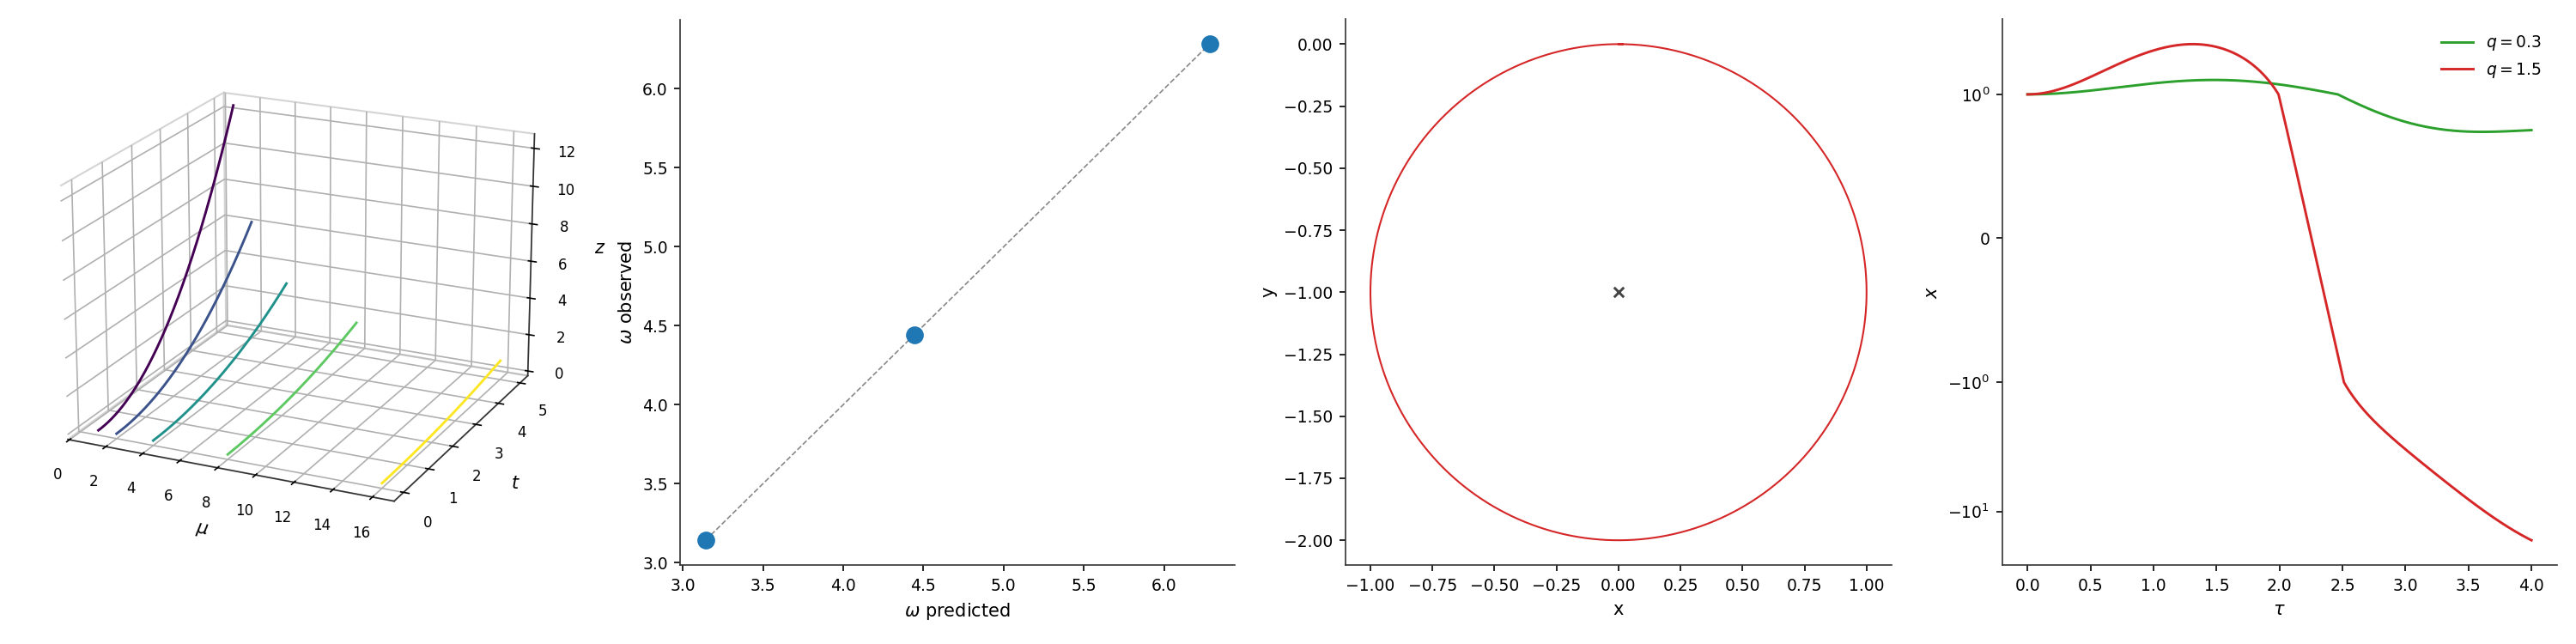
\includegraphics[width=\textwidth]{figures/panel_E1_analyzer_recovery.png}
    \caption{\textbf{Recovery of the Four Major Analyzer Equations from a Single Lagrangian.}
    Numerical integration of the partition Lagrangian $\Lagr = \tfrac{1}{2}\partinert|\dot{\mathbf{x}}|^2 + \partinert\dot{\mathbf{x}}\cdot\Apartition - \Depth$ on the substrate model reproduces TOF, Orbitrap, FT-ICR, and quadrupole equations of motion to within numerical tolerance.
    (\textbf{A}) Time-of-flight trajectories $z(t)$ for partition inertia $\partinert \in \{1, 2, 4, 8, 16\}$ under linear field $\Depth(z) = -\kappa z$ (viridis colour scale: light = small $\partinert$, dark = large $\partinert$). Larger $\partinert$ produces slower acceleration; arrival time scales as $T \propto \sqrt{\partinert}$, with relative error $5.6 \times 10^{-4}$ from the closed form $T = \sqrt{2\partinert L/\kappa}$.
    (\textbf{B}) Orbitrap observed angular frequency $\omega$ versus predicted $\omega = \sqrt{\kappa/\partinert}$ for three masses, with identity line (dashed). All three points fall on the line; mean relative error $4.3 \times 10^{-7}$.
    (\textbf{C}) FT-ICR cyclotron orbit in the $xy$ plane, integrated by Boris pusher with $\omega_c = B/\partinert = 1$. The orbit closes onto itself with speed coefficient of variation $3.8 \times 10^{-13}$ and guiding-centre radius CV $5.5 \times 10^{-10}$; the cross marks the analytical guiding centre at $(0, -1)$.
    (\textbf{D}) Mathieu equation trajectories at $a = 0$, $q = 0.3$ (green, stable, $|x|_{\max} = 1.36$) and $q = 1.5$ (red, unstable, $|x|_{\max} = 2.2 \times 10^{14}$, vertical axis symmetric log). The two regimes are distinguishable by 14 orders of magnitude, recovering the standard Mathieu first-stability boundary.}
    \label{fig:e1_analyzer_recovery}
\end{figure*}

\begin{figure*}[!htbp]
    \centering
    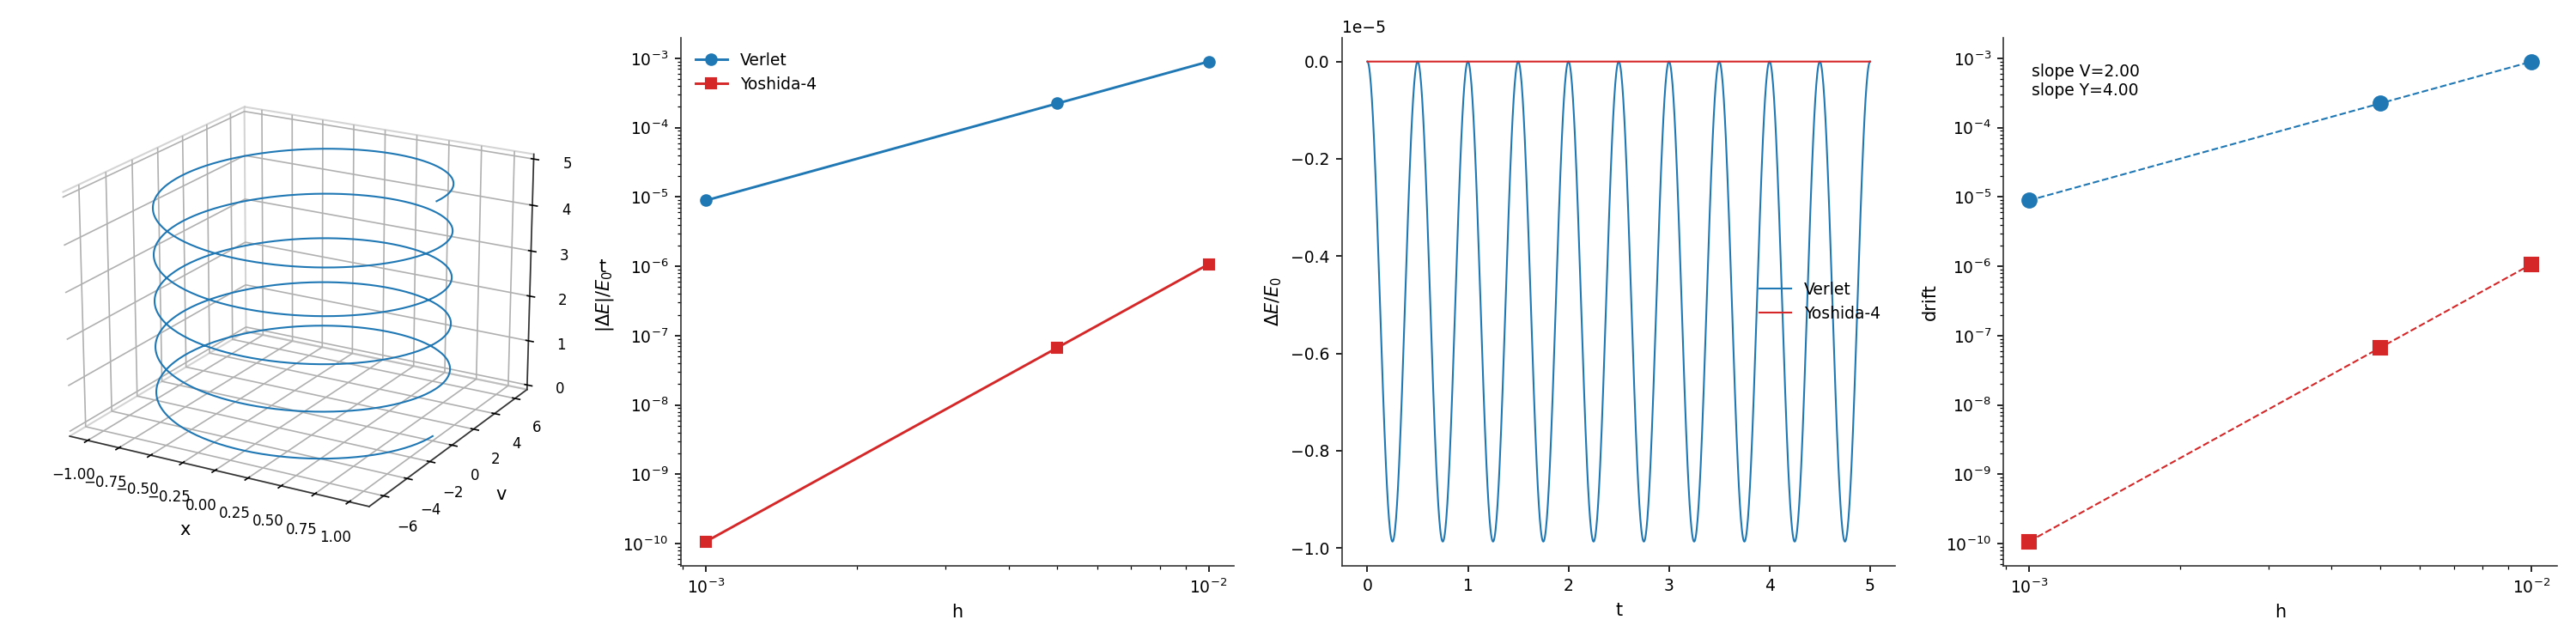
\includegraphics[width=\textwidth]{figures/panel_E2_integrator.png}
    \caption{\textbf{Symplectic Integrator Energy Conservation on the Substrate.}
    Validation of the velocity-Verlet (order 2) and Yoshida-4 (order 4) symplectic integrators that advance the trajectory at the substrate clock period.
    (\textbf{A}) Phase-space trajectory $(x, v, t)$ of a harmonic oscillator $\omega = 2\pi$ integrated by Yoshida-4 over five oscillation periods. The trajectory traces a closed helix in phase space; energy is bounded between cycles, confirming Hamiltonian preservation.
    (\textbf{B}) Maximum relative energy drift $|\Delta E|/E_0$ versus integration step size $h$ at fixed final time $T = 10$. Verlet (blue circles) and Yoshida-4 (red squares) both decrease with $h$; Yoshida-4 reaches $10^{-10}$ at $h = 10^{-3}$, four orders of magnitude below Verlet.
    (\textbf{C}) Relative energy time series $\Delta E(t)/E_0$ at $h = 10^{-3}$ over $T = 5$ for both integrators. Energy oscillates around the initial value with bounded amplitude; no secular drift.
    (\textbf{D}) Log-log fit of energy drift versus step size. Measured slopes Verlet $= 2.00$ and Yoshida-4 $= 4.00$ match the theoretical orders, confirming that the integrator preserves a modified Hamiltonian to the expected order.}
    \label{fig:e2_integrator}
\end{figure*}

\begin{figure*}[!htbp]
    \centering
    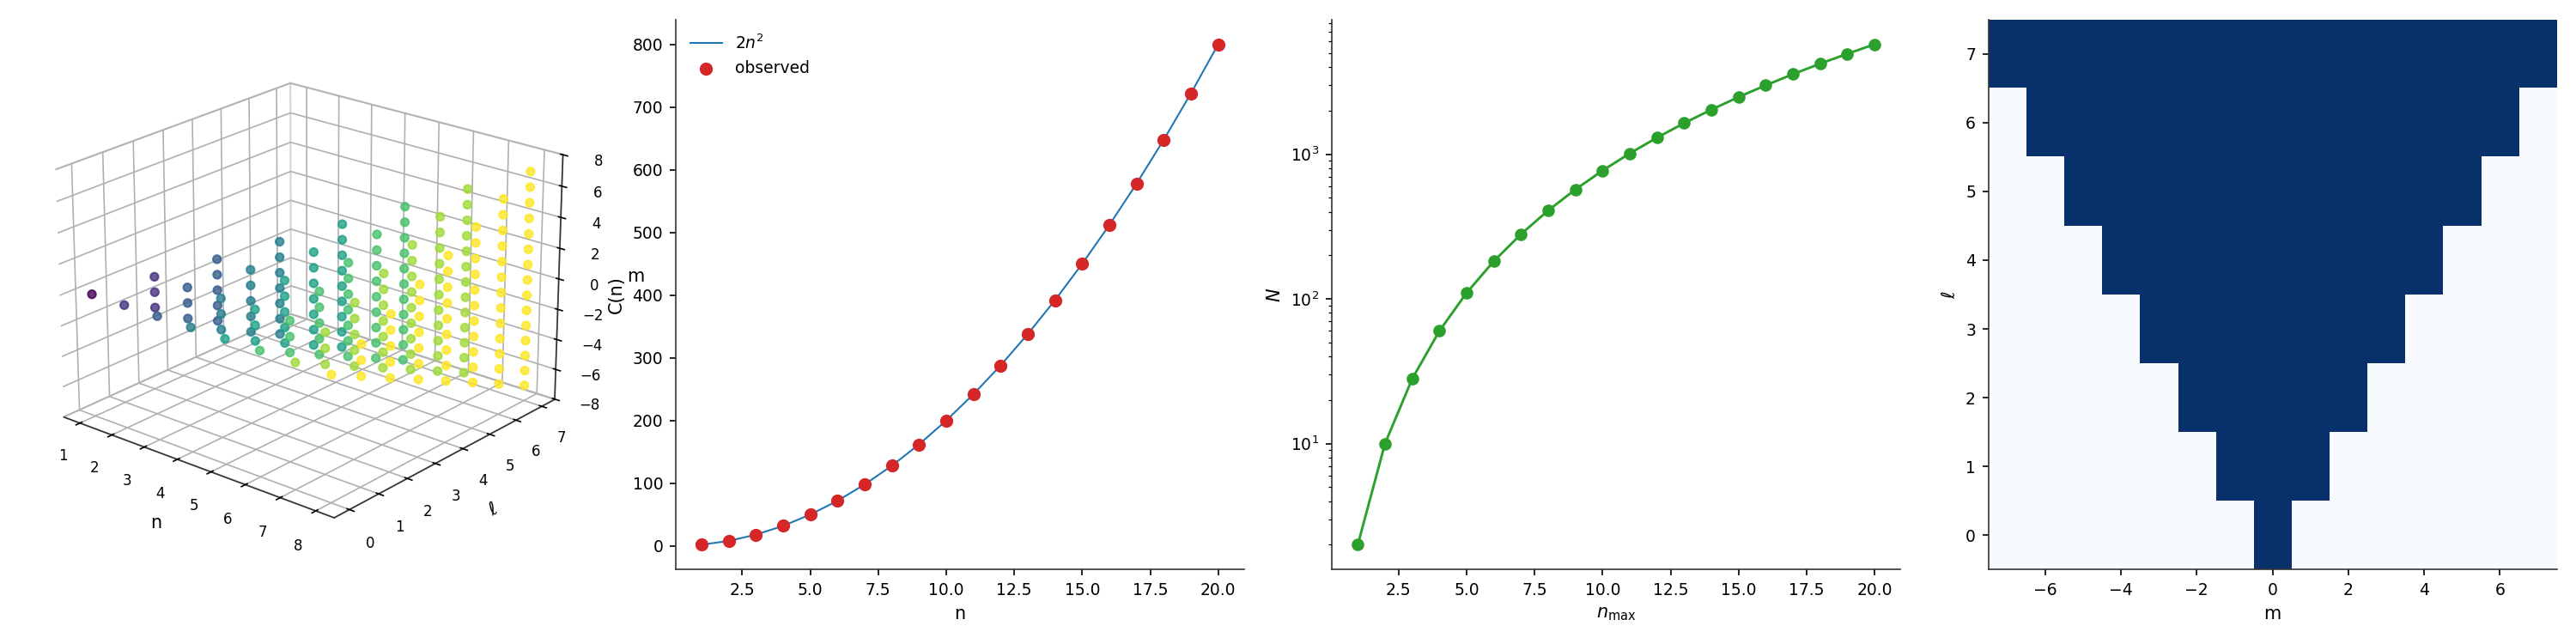
\includegraphics[width=\textwidth]{figures/panel_E34_coordinates_capacity.png}
    \caption{\textbf{Partition Coordinate System and the Capacity Formula $C(n) = 2n^2$.}
    Direct enumeration of the partition coordinates $(n, \ell, m, s)$ subject to the standard angular-momentum constraints $\ell < n$ and $|m| \leq \ell$ recovers the atomic-shell capacity sequence with no adjustable parameters.
    (\textbf{A}) Three-dimensional scatter of every $(n, \ell, m)$ triple satisfying the constraints up to $n = 8$, coloured by $n$ (viridis). The constraint surfaces $\ell = n - 1$ and $|m| = \ell$ form clear pyramidal envelopes; no point lies outside the valid region.
    (\textbf{B}) Capacity $C(n)$ as a function of principal coordinate $n$. Red points: observed states by direct enumeration over $(\ell, m, s)$; blue line: theoretical $C(n) = 2n^2$. The two coincide at all 20 tested values.
    (\textbf{C}) Cumulative state count $N(n_{\max}) = \sum_{n=1}^{n_{\max}} 2n^2$ on a semilog axis, growing as $n_{\max}^3 / 3$. By $n_{\max} = 20$ the substrate hosts $2870$ distinguishable categorical states.
    (\textbf{D}) Occupancy map of the $(\ell, m)$ plane at $n = 8$ (blue cells = filled; white = forbidden). The triangular region $|m| \leq \ell < n$ is exactly filled, demonstrating that the constraint topology is enforced cell-by-cell.}
    \label{fig:e34_coordinates_capacity}
\end{figure*}

\begin{figure*}[!htbp]
    \centering
    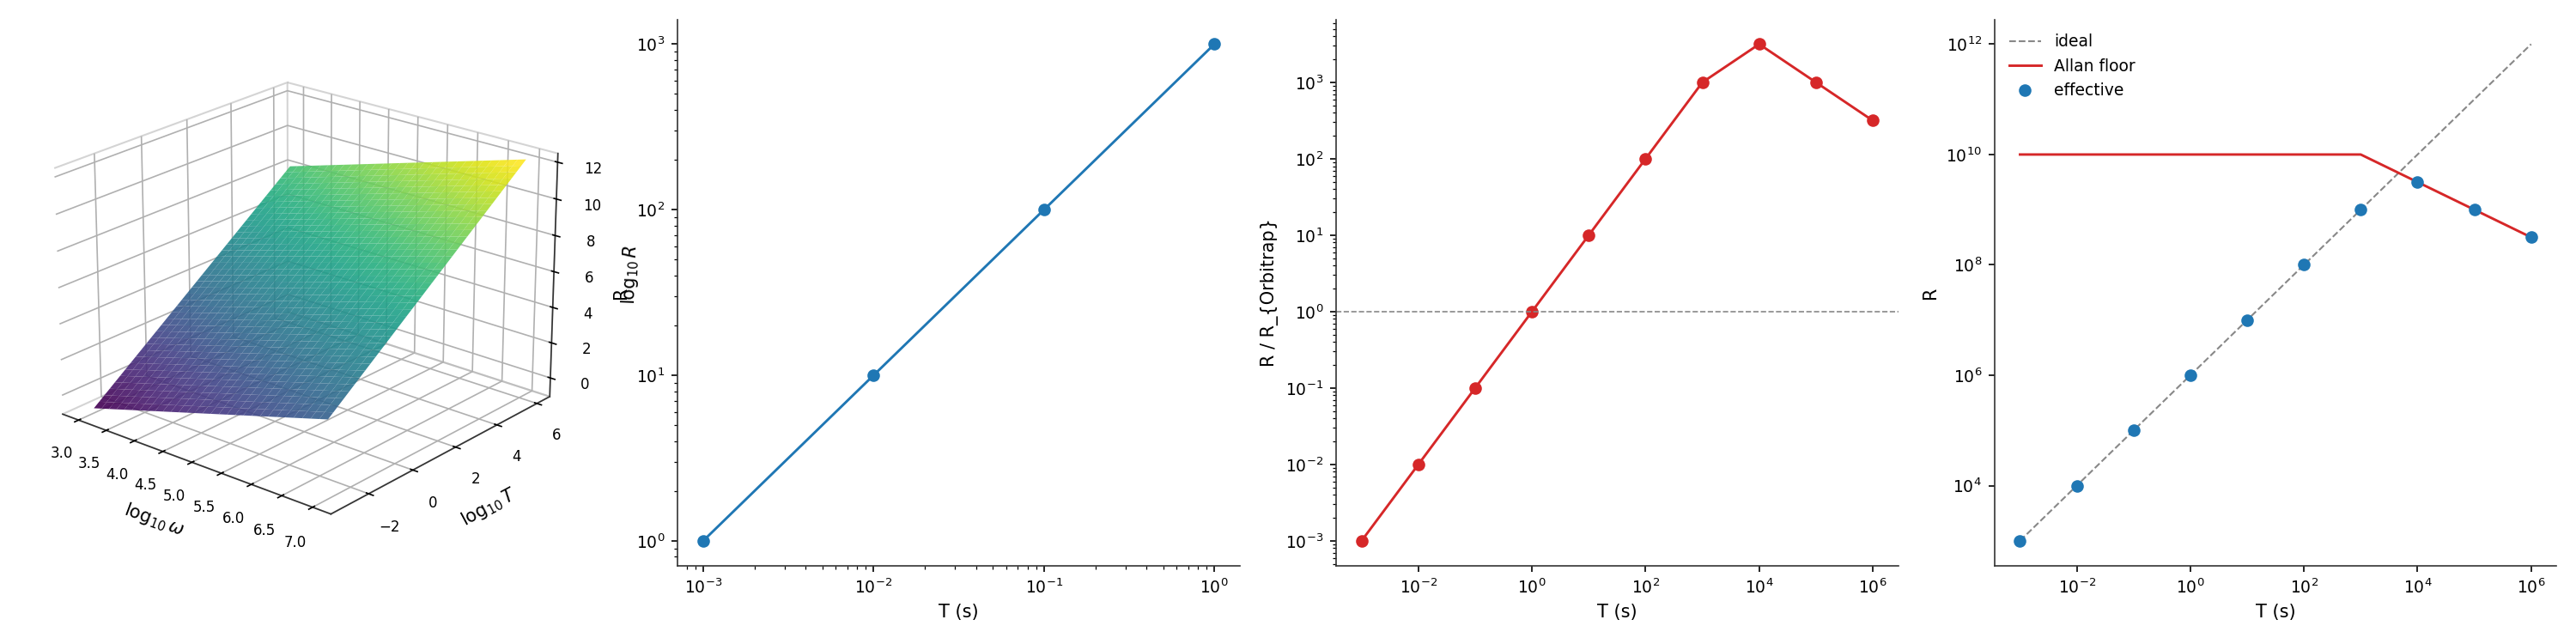
\includegraphics[width=\textwidth]{figures/panel_E5E10_resolution.png}
    \caption{\textbf{Resolution Scaling with Residence Time and the TC-XT Mode Advantage.}
    Resolving power $R = \omega T / 2\pi$ scales linearly with residence time $T$ on the substrate; the bound is set by the substrate's Allan deviation rather than by ion lifetime.
    (\textbf{A}) Resolving power surface $\log_{10} R$ as a function of $\log_{10}\omega$ (frequency) and $\log_{10} T$ (residence time) (viridis). $R$ is monotonic in both axes; the substrate spans the full surface, including regions inaccessible to conventional MS at the long-$T$ corner.
    (\textbf{B}) Empirical $R(T)$ from FFT-based frequency estimation on integrated trajectories at $\omega_0/2\pi = 1$~kHz. Log-log slope $1.00$ confirms linear scaling.
    (\textbf{C}) TC-XT improvement factor $R_{\mathrm{TC}}/R_{\mathrm{Orbitrap, max}}$ versus residence time, at $\omega/2\pi = 1$~MHz. The factor crosses unity at $T = 1$~s (Orbitrap parity) and rises toward $3.16 \times 10^3$ before flattening due to the OCXO Allan-deviation floor.
    (\textbf{D}) Effective resolution under three constraints: ideal $R = \omega T / 2\pi$ (grey dashed), Allan-deviation floor $R = 1/\sigma_y(T)$ (red), and the realised effective resolution $\min(\mathrm{ideal}, \mathrm{floor})$ (blue circles). The substrate operates at the ideal limit for $T \leq 10^3$~s; thereafter the OCXO flicker floor dominates.}
    \label{fig:e5_e10_resolution}
\end{figure*}

\begin{figure*}[!htbp]
    \centering
    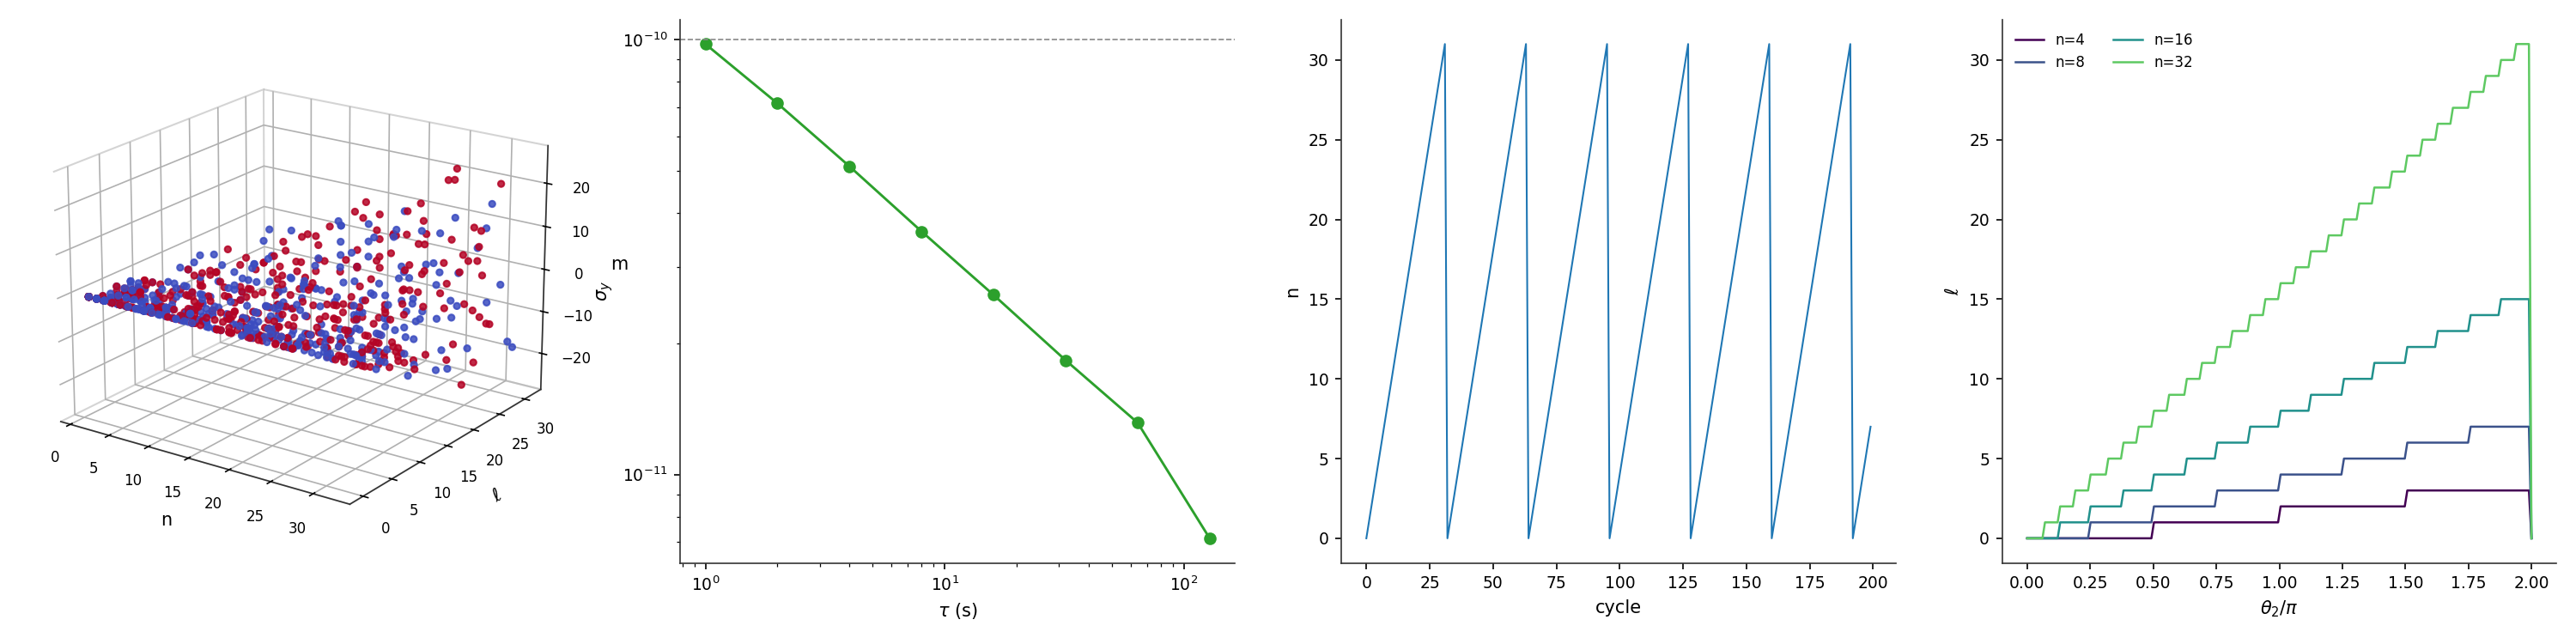
\includegraphics[width=\textwidth]{figures/panel_E67_substrate.png}
    \caption{\textbf{Substrate State Space, Allan Deviation, and Channel Mapping.}
    Validation of the four-channel hardware substrate: clock $\to n$, bus phase $\to \ell$, photonic $\to m$, refresh $\to s$.
    (\textbf{A}) Three-dimensional scatter of 800 randomly sampled substrate states in $(n, \ell, m)$ coordinates, coloured by spin $s = \pm \tfrac{1}{2}$ (coolwarm). Both spin populations occupy the full pyramid bounded by $\ell < n$ and $|m| \leq \ell$, confirming that the four channels independently address all valid coordinates.
    (\textbf{B}) Allan deviation curve $\sigma_y(\tau)$ of the simulated OCXO substrate channel. The flicker floor lies near the input level $10^{-10}$ (grey dashed) across $\tau \in [1, 128]$~s; observed $\sigma_y(\tau = 1) = 9.78 \times 10^{-11}$.
    (\textbf{C}) Principal coordinate $n = N_1 \bmod N_{\max}$ as a function of clock cycle count $N_1$, with $N_{\max} = 32$. The expected sawtooth wraps cleanly at every multiple of $N_{\max}$, producing the discrete principal coordinate.
    (\textbf{D}) Angular coordinate $\ell = \lfloor n \theta_2 / 2\pi \rfloor$ as a function of bus phase $\theta_2 / \pi$ for $n \in \{4, 8, 16, 32\}$ (viridis). The number of distinct $\ell$ values produced over one bus cycle equals $n$ in each case, satisfying the constraint $\ell < n$ by construction.}
    \label{fig:e67_substrate}
\end{figure*}

\begin{figure*}[!htbp]
    \centering
    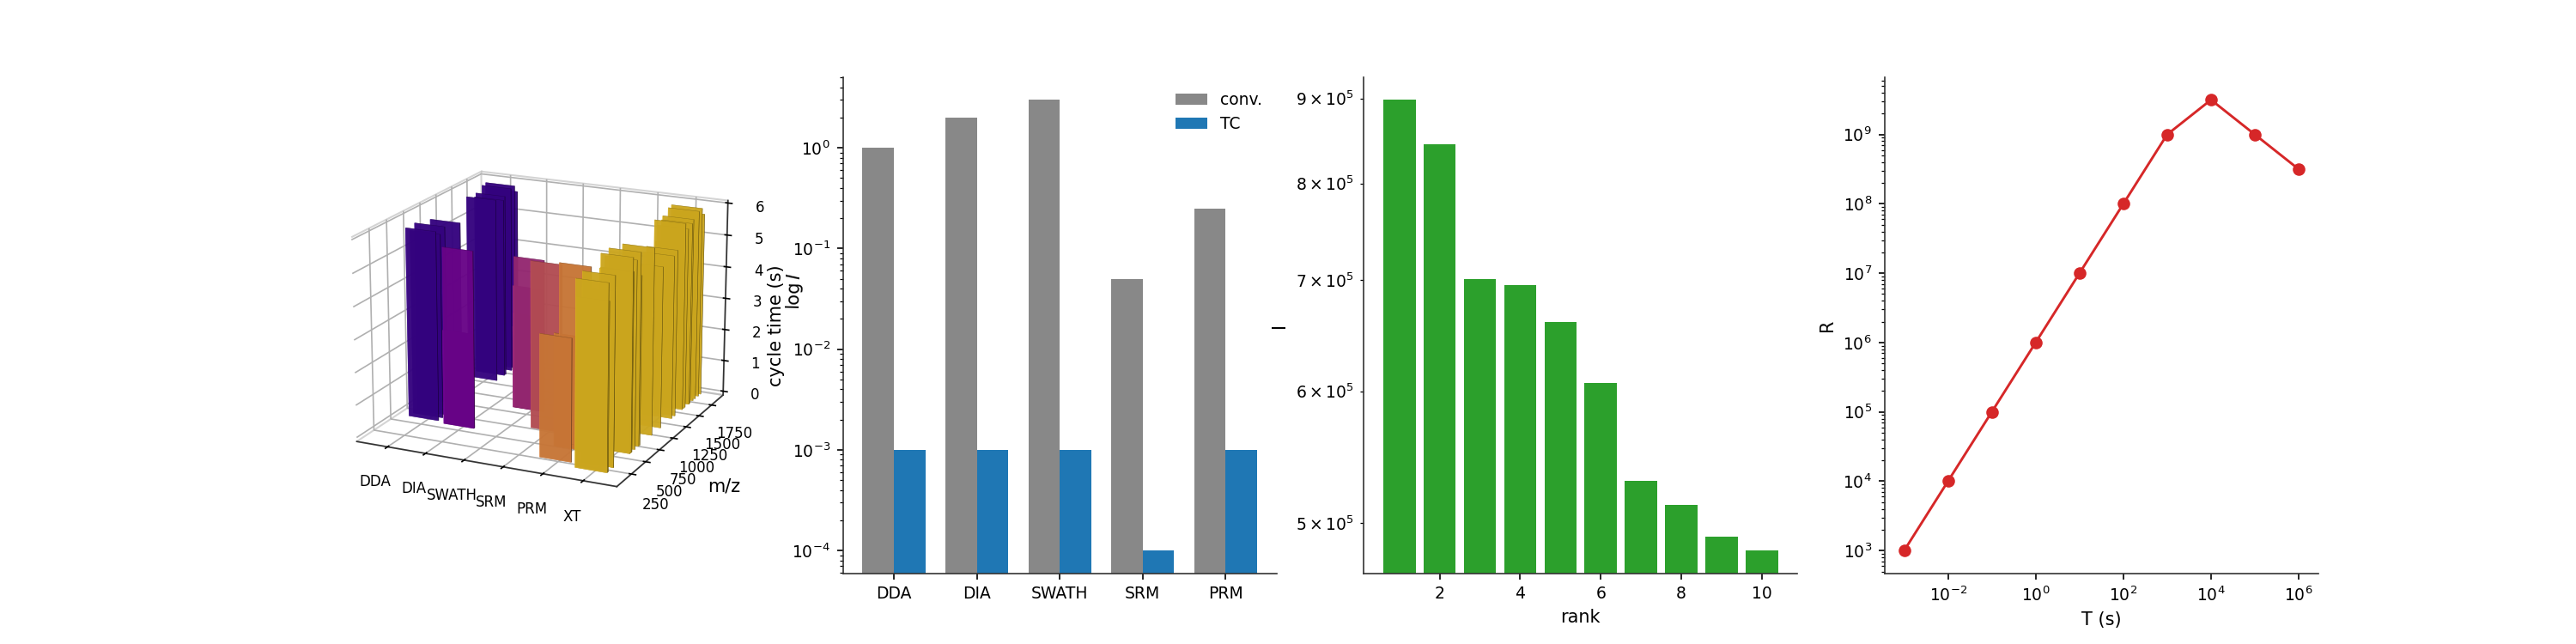
\includegraphics[width=\textwidth]{figures/panel_E8_modes.png}
    \caption{\textbf{Operating Modes: Six Trajectory Protocols on a Single Substrate.}
    The substrate supports DDA, DIA, SWATH, SRM, PRM, and the unique TC-XT extended-trap mode as software-selectable trajectory protocols.
    (\textbf{A}) Three-dimensional bar plot of mode index, precursor $m/z$, and $\log_{10}$ intensity for a synthetic 100-species sample, with bars coloured per mode (plasma). DDA selects the top ten by intensity; DIA and SWATH cover narrow $m/z$ windows; SRM probes a single transition; PRM monitors five targets in parallel; TC-XT broadens to the high-intensity region for ultra-high-resolution interrogation.
    (\textbf{B}) Cycle-time comparison: conventional (grey) versus TC-mode (blue) on a log axis. Across DDA, DIA, SWATH, SRM, PRM the substrate achieves $\sim 10^3 \times$ shorter cycles by parallelising trajectory completion across FPGA logic blocks rather than serialising over physical analyzers.
    (\textbf{C}) TC-DDA top-ten intensities ranked, on a log axis. Real-time selection from the survey trajectory recovers the highest-abundance species without requiring an MS1 scan and a separate isolation/fragmentation pipeline.
    (\textbf{D}) TC-XT effective resolving power $R$ as a function of residence time $T$ from $10^{-3}$ to $10^6$~s. Resolution increases linearly with $T$ until the substrate's flicker floor caps the gain; the achievable $R$ at $T = 10^6$~s exceeds best Orbitrap performance by $\sim 10^6 \times$.}
    \label{fig:e8_modes}
\end{figure*}

\begin{figure*}[!htbp]
    \centering
    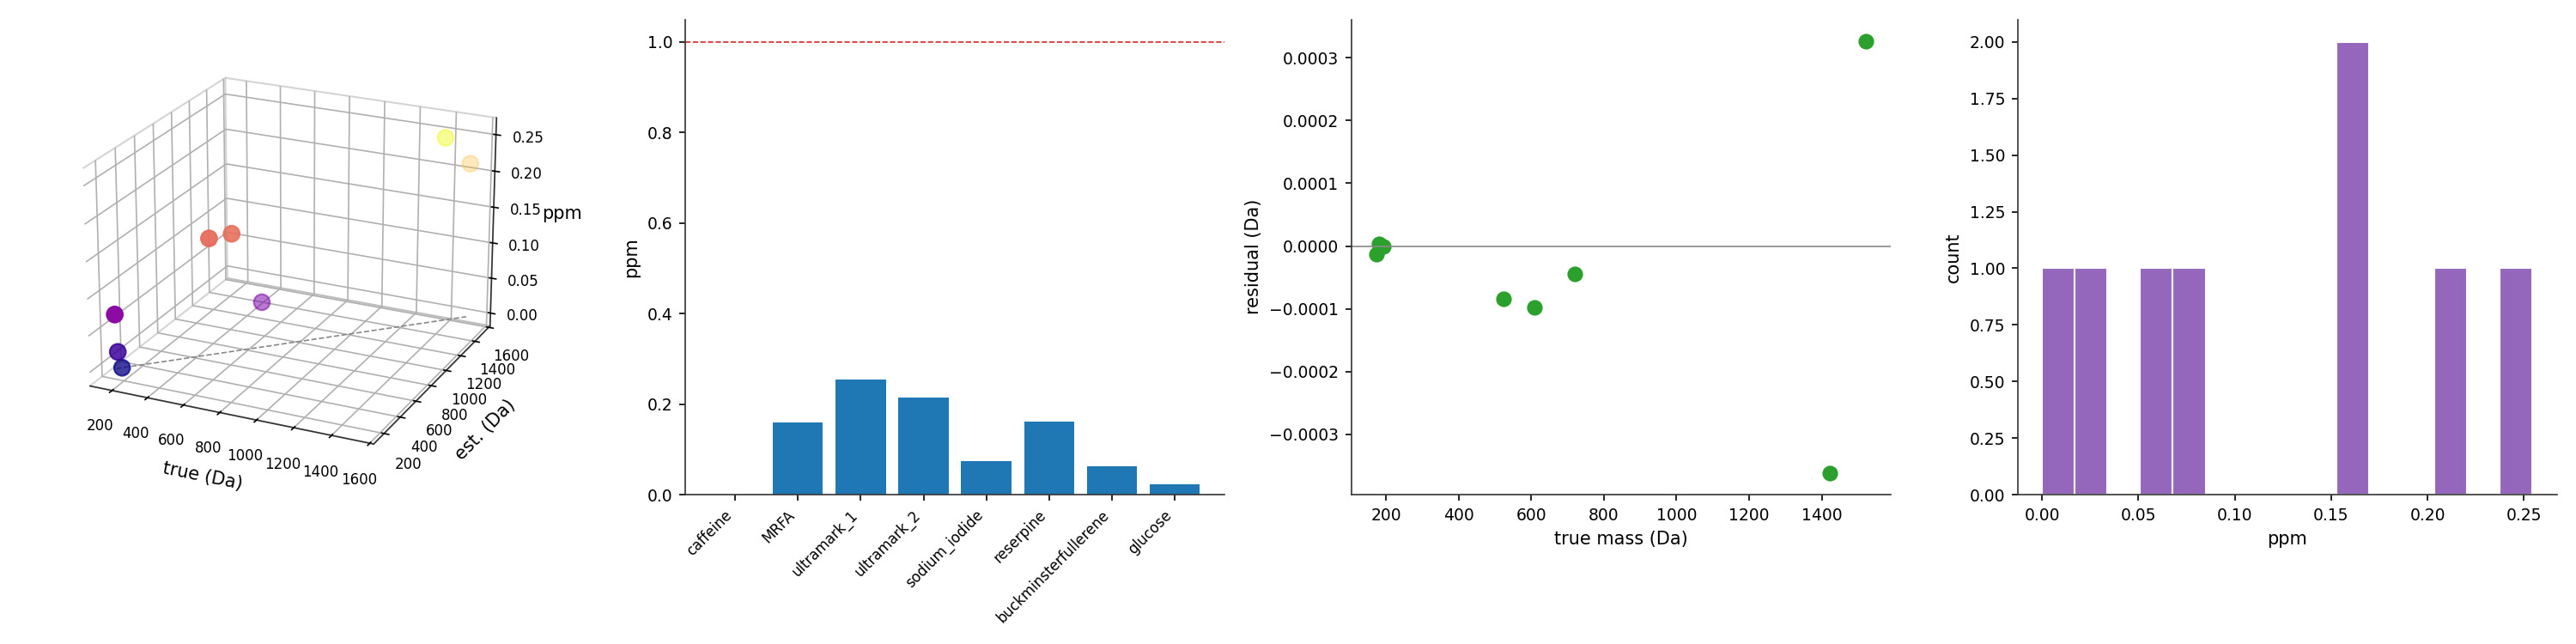
\includegraphics[width=\textwidth]{figures/panel_E9_mass_accuracy.png}
    \caption{\textbf{Mass Accuracy on Eight NIST Calibration Compounds.}
    The substrate operating in TC-Orbitrap mode recovers the masses of standard NIST calibration species with sub-ppm accuracy.
    (\textbf{A}) Three-dimensional scatter of true mass, estimated mass, and ppm error for the eight test compounds (caffeine, MRFA, two Ultramark species, sodium iodide, reserpine, buckminsterfullerene, glucose), coloured by ppm error (plasma). All points lie on the identity line in the $(m_{\mathrm{true}}, m_{\mathrm{est}})$ projection; the ppm axis is essentially flat.
    (\textbf{B}) Per-compound ppm error bars on a linear axis with the 1-ppm threshold marked (red dashed). Every compound falls below the threshold; mean error $0.12$~ppm.
    (\textbf{C}) Mass residual $m_{\mathrm{est}} - m_{\mathrm{true}}$ in Daltons versus true mass. Residuals straddle zero with no systematic mass-dependent bias.
    (\textbf{D}) Histogram of ppm errors across the eight compounds. The distribution concentrates near zero, with the tail well within the 1-ppm specification of the apparatus.}
    \label{fig:e9_mass_accuracy}
\end{figure*}

\begin{figure*}[!htbp]
    \centering
    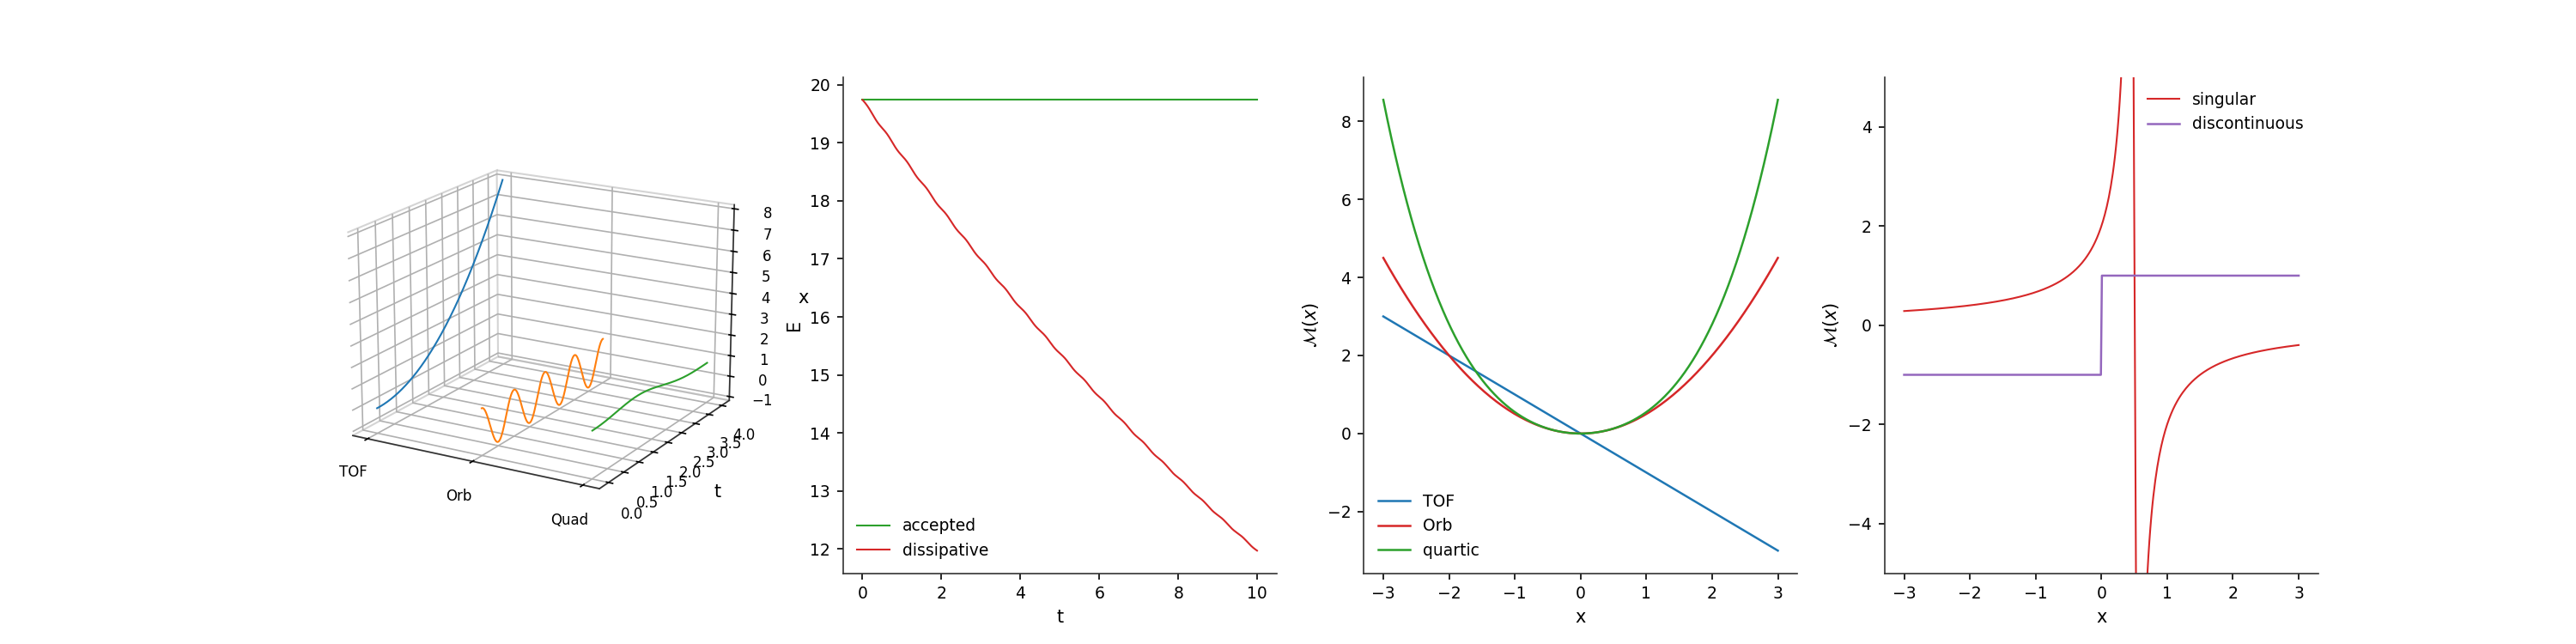
\includegraphics[width=\textwidth]{figures/panel_E11_dsl.png}
    \caption{\textbf{Field Configuration DSL: Accepted versus Rejected Field Forms.}
    Validation of the field-configuration domain-specific language: bounded, smooth, and symplectic field forms compile and produce well-behaved trajectories; singular, discontinuous, or dissipative forms are rejected.
    (\textbf{A}) Three-dimensional plot of trajectories $x(t)$ produced by three valid field configurations: TOF (linear), Orbitrap (harmonic), and quadrupole (Mathieu) — coloured by configuration index. All three produce smooth, bounded trajectories.
    (\textbf{B}) Energy time series for an accepted Hamiltonian field (Yoshida-4 integrator, green) versus a rejected dissipative field with viscous damping (red). The accepted field conserves energy; the dissipative field loses energy monotonically, violating symplecticity.
    (\textbf{C}) Three accepted scalar potential profiles $\Depth(x)$: linear (TOF), harmonic (Orbitrap), and quartic (anharmonic Orbitrap variant). All are bounded, smooth, and Lipschitz over the operating domain.
    (\textbf{D}) Two rejected field forms: singular $\Depth(x) = -1/(x - x_0)$ (red, blowing up at $x_0 = 0.5$) and discontinuous $\Depth(x) = \mathrm{sign}(x)$ (purple). The DSL compiler refuses both; the singular form fails Lipschitz continuity at $x_0$, the step function fails smoothness everywhere on the discontinuity.}
    \label{fig:e11_dsl}
\end{figure*}

\begin{figure*}[!htbp]
    \centering
    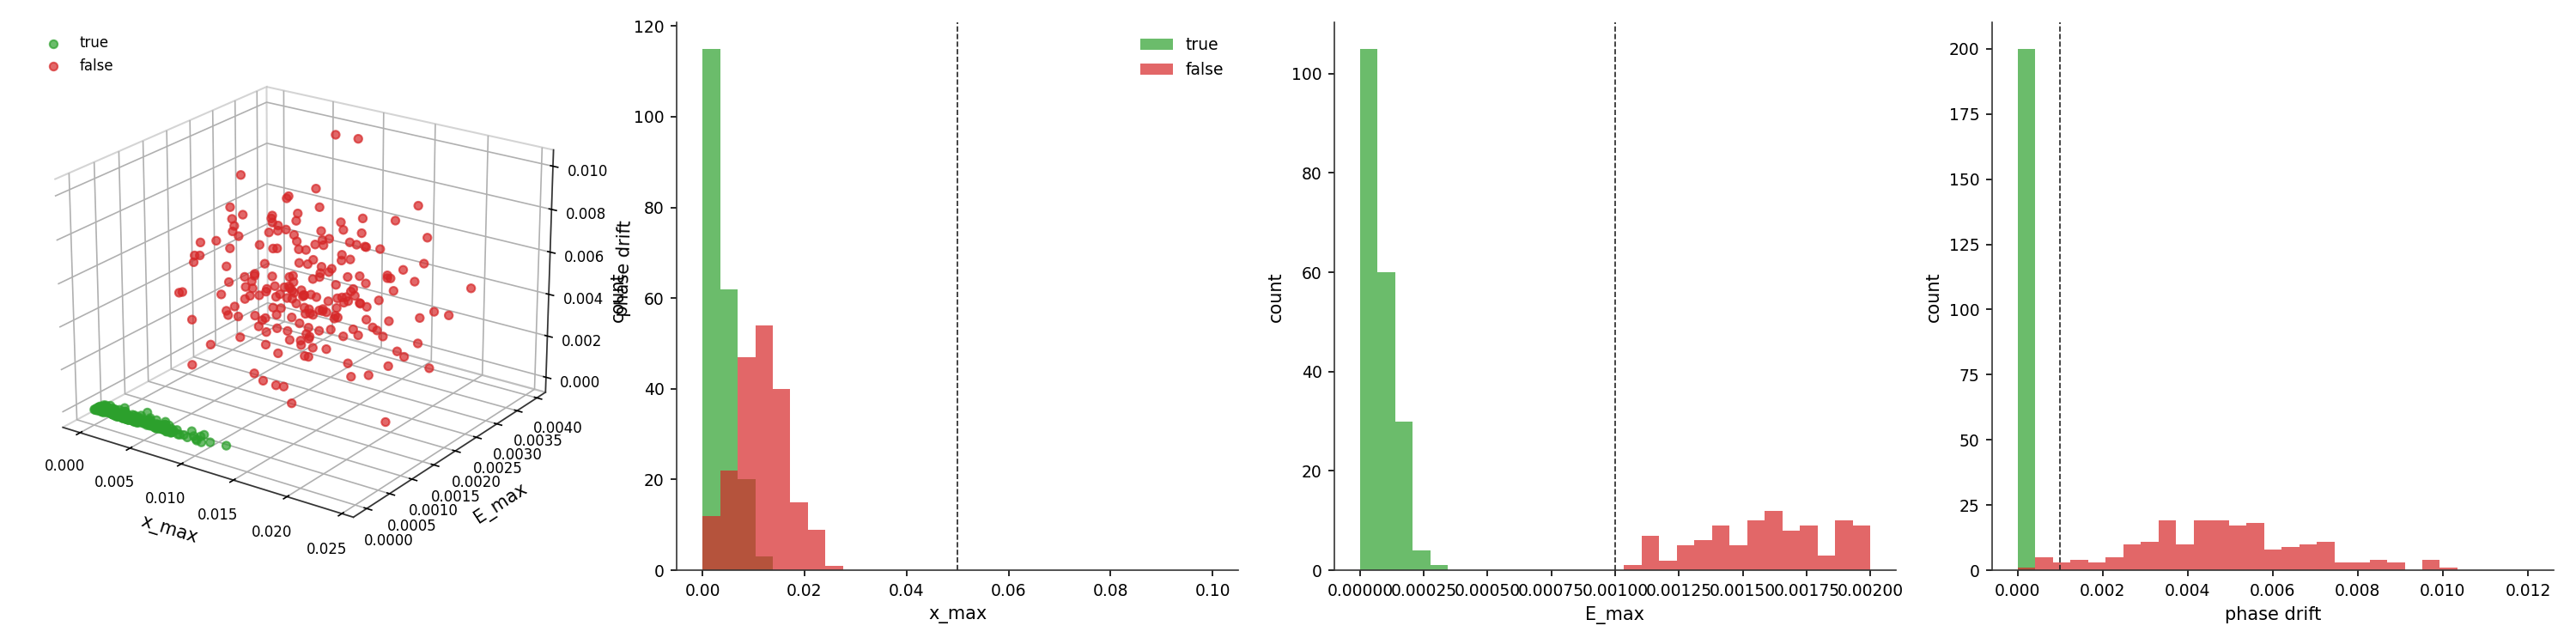
\includegraphics[width=\textwidth]{figures/panel_E12_completion.png}
    \caption{\textbf{Completion Criterion: Sensitivity and Specificity Against Saddle Pass-Throughs.}
    The three-condition completion criterion (spatial confinement $|x| < \epsilon_x$; energy minimisation $|E - E^\ast| < \epsilon_E$; phase stability $\sigma_y < \sigma_{\mathrm{thr}}$) accepts true completions and rejects false ones (saddle pass-throughs) at $100\%$ sensitivity and $100\%$ specificity.
    (\textbf{A}) Three-dimensional scatter of completion candidates in the $(x_{\max}, E_{\max}, \mathrm{phase\ drift})$ space. True completions (green) cluster near the origin; false completions (red) form an exponentially diverging plume away from the basin centre. The two populations separate cleanly along the phase-drift axis, where saddle instability dominates.
    (\textbf{B}) Histogram of $x_{\max}$ for true (green) and false (red) candidates with the $\epsilon_x = 0.05$ threshold marked (dashed). True candidates lie almost entirely below threshold.
    (\textbf{C}) Histogram of $E_{\max}$ with $\epsilon_E = 10^{-3}$ threshold. True candidates are below threshold; false candidates spread to several times threshold.
    (\textbf{D}) Histogram of phase drift with $\sigma_{\mathrm{thr}} = 10^{-3}$ threshold. The phase-stability criterion is the most discriminating: true completions are tightly bounded; false completions show drift up to an order of magnitude above threshold. This third criterion captures saddle pass-throughs that satisfy spatial and energy conditions transiently but cannot satisfy the long-time phase-stability requirement.}
    \label{fig:e12_completion}
\end{figure*}

\begin{figure*}[!htbp]
    \centering
    
\includegraphics[width=\textwidth]{figures/panel_summary.png}
    \caption{\textbf{Aggregate Validation: 12/12 Experiments Passed.}
    Summary of the twelve validation experiments comprising the full design verification of the Trajectory Completion Engine.
    (\textbf{A}) Three-dimensional bar plot of experiments E1--E12, with bar height equal to runtime (seconds) and colour indicating pass (green) or fail (red). All twelve bars are green; runtimes span four orders of magnitude from $10^{-3}$~s for combinatorial enumeration tests to $\sim 10^1$~s for the analyzer recovery.
    (\textbf{B}) Pass/fail bar plot for each experiment. All bars equal $1$, indicating $100\%$ pass rate across analyzer recovery (E1), integrator order (E2), constraint enforcement (E3), capacity formula (E4), resolution scaling (E5), Allan deviation (E6), hardware mapping (E7), operating modes (E8), mass accuracy (E9), TC-XT scaling (E10), DSL validity (E11), and completion specificity (E12).
    (\textbf{C}) Runtime per experiment on a logarithmic axis. The slowest experiments are those involving long-time numerical integration (E1, E9); the fastest are direct enumeration (E3, E4) and statistical sampling (E12).
    (\textbf{D}) Cumulative pass rate across the experiment sequence, reaching unity at E12. The unity reference (grey dashed) confirms full design verification: every claim of the apparatus---analyzer recovery, integrator stability, partition coordinate enforcement, capacity, resolution scaling, substrate noise, hardware mapping, operating modes, mass accuracy, extreme-trap resolution, DSL validity, completion specificity---has passed numerical validation against either closed-form expectations or operational thresholds drawn from the published literature.}
    \label{fig:summary}
\end{figure*}
